% =====================================================================
% Guía del estudiante -- Álgebra 8° -- Trimestre I
% María Mercedes Cantillo · Colegio San Alberto Magno
% ---------------------------------------------------------------------
% Hilo conductor: La cacería de π
% Plan (etapas A y B): guia-periodo-I-numeros-irracionales.plan.md
% Temas (de curriculo/programacion.csv, sesiones 007-033):
%   racionalesirracionales, escandalopitagorico, irracionalesvidareal,
%   radicalesaplicaciones
% Cada \tema tiene \label{tema:...} para que las clases lo citen con
% \refguia{tema:...}. No borrar el .aux de esta guía.
% Ejercicios: recursos/banco/matematicas/irracionales-8.py y los reusados
% (numeros-reales-8, radicacion-8, medidas-con-radicales-8).
%
% Compilar:  latexmk -pdf guia-periodo-I-numeros-irracionales.tex
% =====================================================================
\documentclass[11pt]{article}
\makeatletter\def\input@path{{../../../../plantillas/estilo/}}\makeatother
\usepackage{mmcantillo}

% ======================== DATOS DE LA GUÍA ============================
\tipodocumento{Guía del estudiante}
\asignatura{Álgebra}
\titulo{La cacería de $\pi$}
\grado{8°}
\periodo{I}
\hiloconductor{La cacería de $\pi$: del papiro Rhind a Lambert}
% ======================================================================
% DBA: matematicas grado 8 · DBA 1 — Reconoce la existencia de los números
%      irracionales como números no racionales y los describe de acuerdo
%      con sus características y propiedades.
%      DBA 2 — Construye representaciones, argumentos y ejemplos de
%      propiedades de los números racionales y no racionales.

\newcommand{\I}{\mathbb{I}}

\begin{document}

\encabezado

% ---------------------------------------------------------------------
% 1. Frase introductoria
% ---------------------------------------------------------------------
% verificado: https://books.google.com/books/about/Grundlagen_einer_allgemeinen_Mannichfalt.html?id=1LPOSWUtK4UC — Cantor, Grundlagen (Teubner, 1883), §8: «das Wesen der Mathematik liegt gerade in ihrer Freiheit»; Gesammelte Abhandlungen (1932), p. 182 (ubicado con https://de.wikiquote.org/wiki/Georg_Cantor)
\frase{La esencia de la matemática está precisamente en su libertad.}
{Georg Cantor, \emph{Fundamentos de una teoría general de conjuntos} (1883), §8 (trad. propia)}

% ---------------------------------------------------------------------
% 2. Introducción
% ---------------------------------------------------------------------
\seccion{Introducción}

Toma cualquier objeto redondo —una moneda, una tapa, la llanta de una
bicicleta— y mide con una cuerda su borde y su diámetro. Siempre pasará lo
mismo: el borde mide un poco más de tres veces el diámetro. Ese «un poco más
de tres» es el número $\pi$, y la humanidad lleva cuatro mil años
persiguiéndolo. Durante casi todo ese tiempo se creyó que $\pi$, como
cualquier medida, se podía escribir como una fracción: el problema era solo
encontrarla.

Este trimestre seguiremos esa cacería. Veremos por qué algunas fracciones se
convierten en decimales que se repiten para siempre, cómo los griegos
descubrieron un número que no es fracción —la diagonal de un cuadrado—, cómo
Arquímedes encerró a $\pi$ entre dos polígonos usando raíces cuadradas, y
cómo, en 1761, se demostró por fin que ninguna fracción es igual a $\pi$.

\textbf{Al terminar este trimestre podrás:}
\begin{itemize}
  \item distinguir un número racional de uno irracional por su expresión
        decimal, y pasar un decimal periódico a fracción;
  \item argumentar por qué $\sqrt{2}$ y otros números no son racionales, y
        construirlos y ubicarlos en la recta numérica;
  \item representar un mismo número de varias maneras (geométrica, decimal,
        como fracción o como raíz) y clasificarlo en $\N$, $\Z$, $\Q$, $\I$ o $\R$;
  \item simplificar y aproximar radicales para resolver problemas de medidas.
\end{itemize}

Este trimestre trabaja dos Derechos Básicos de Aprendizaje del Ministerio de
Educación Nacional~\cite{mendba}:

\begin{dba}[Grado 8° · DBA 1]
Reconoce la existencia de los números irracionales como números no
racionales y los describe de acuerdo con sus características y propiedades.
\end{dba}

\begin{dba}[Grado 8° · DBA 2]
Construye representaciones, argumentos y ejemplos de propiedades de los
números racionales y no racionales.
\end{dba}

% ---------------------------------------------------------------------
% 3. Marco teórico
% ---------------------------------------------------------------------
\seccion{Marco teórico}

\subsubsection*{Un número conocido desde siempre}

Cualquier círculo, grande o pequeño, cumple lo mismo: su circunferencia
dividida entre su diámetro da siempre el mismo número, $\pi$. En el papiro
Rhind, copiado en Egipto hacia el año 1650 a.\,C., el área de un círculo se
calcula de una manera que equivale a usar $\pi \approx 3{,}16$~\cite{mactutorpi}.
Durante miles de años nadie dudó de que $\pi$ se pudiera escribir como una
fracción; faltaba encontrarla.

\subsubsection*{«Todo es número»}

En el siglo VI a.\,C., en el sur de Italia, los pitagóricos pensaban que los
principios de los números eran los principios de todas las
cosas~\cite{aristoteles}: cualquier longitud, y cualquier relación entre
longitudes, debía poder escribirse como una razón entre números enteros —lo
que hoy llamamos un número \textbf{racional}—. Lo comprobaban en la música:
dos cuerdas iguales suenan a una octava de distancia cuando sus longitudes
están en razón $2:1$.

\subsubsection*{El primer número que no es fracción}

Esa convicción se rompió con una figura mucho más sencilla que el círculo:
la diagonal de un cuadrado no es conmensurable con su lado; en lenguaje de
hoy, $\sqrt{2}$ no es racional. No sabemos quién lo descubrió. Autores
antiguos tardíos cuentan que el pitagórico que reveló el secreto murió en el
mar, y la tradición posterior le puso el nombre de Hipaso de Metaponto, pero
ninguna fuente antigua lo liga directamente con este
descubrimiento~\cite{huffman}. Lo que sí sabemos es que en el siglo IV
a.\,C. la demostración ya circulaba: Aristóteles la pone como ejemplo de
razonamiento por el absurdo.

% verificado: https://www.tau.ac.il/~corry/publications/articles/Narrative/notes/aristo.html — Aristóteles, Primeros analíticos I.23 (41a26-27): la diagonal es inconmensurable porque, si se supone conmensurable, los impares resultan iguales a los pares
\begin{cita}{Aristóteles, \emph{Primeros analíticos} I.23, 41a26--27 (trad. propia)~\cite{corry}}
La diagonal del cuadrado es inconmensurable con el lado, porque, si se
supone conmensurable, los impares resultan iguales a los pares.
\end{cita}

Poco después, según cuenta Platón en el \emph{Teeteto}, Teodoro de Cirene
demostraba lo mismo para las raíces de $3$, de $5$ y así, una por una, hasta
la de $17$~\cite{mactutortheodorus}. Hacia el 300 a.\,C., Euclides dedicó el
Libro X de sus \emph{Elementos} —el más extenso de los trece, con 115
proposiciones— a las magnitudes inconmensurables~\cite{euclides}. Si
$\sqrt{2}$ no era una fracción, ¿lo sería $\pi$?

\subsubsection*{Arquímedes encierra a $\pi$}

Hacia el 250 a.\,C., Arquímedes de Siracusa no intentó escribir $\pi$
exactamente: lo \emph{encerró}. Dibujó un polígono regular de 96 lados
dentro de un círculo y otro por fuera; el perímetro del de adentro es menor
que la circunferencia, y el del de afuera, mayor. Así demostró que
$\frac{223}{71} < \pi < \frac{22}{7}$, es decir, que $\pi$ está entre
$3{,}1408$ y $3{,}1429$~\cite{mactutorpi}. Para lograrlo tuvo que aproximar
raíces cuadradas, como $\sqrt{3}$, sin explicar nunca cómo lo
hizo~\cite{arqraices}. Por eso $\frac{22}{7}$ sigue siendo la aproximación
escolar de $\pi$.

\subsubsection*{Hipatia}

Hacia el año 400, en Alejandría —la ciudad de Euclides—, \textbf{Hipatia}
dirigía una escuela donde enseñaba matemáticas y filosofía; las fuentes
antiguas le atribuyen comentarios a la \emph{Aritmética} de Diofanto y a las
\emph{Cónicas} de Apolonio. Es la primera mujer de la que sabemos con
seguridad que hizo un aporte importante a las matemáticas, sobre todo
conservando y enseñando la obra de los griegos~\cite{dzielska}.

\subsubsection*{355/113}

En China, Zu Chongzhi (430--501) dio el valor $\frac{355}{113} =
3{,}1415929\ldots$, que coincide con $\pi$ en sus primeras seis cifras
decimales~\cite{mactutorpi}.

\subsubsection*{Fin de la cacería… y otra que empieza}

Tanta precisión hacía sospechar que $\pi$ no era ninguna fracción, pero
sospechar no es demostrar. En 1761, Johann Heinrich Lambert presentó ante la
Academia de Berlín la demostración de que $\pi$ es irracional; su memoria se
publicó en 1768~\cite{lambert}. Desde entonces sabemos que su decimal nunca
termina ni se repite. La cacería cambió de presa: ya no se busca la fracción
de $\pi$, sino más cifras. En noviembre de 2025, un solo servidor terminó de
calcular 314 billones de cifras decimales de $\pi$ después de 110 días de
trabajo~\cite{storagereview}.

% ---------------------------------------------------------------------
% 4. Temas
% ---------------------------------------------------------------------
\tema{De los racionales a los irracionales}\label{tema:racionalesirracionales}

\begin{hilo}
Durante milenios se buscó la fracción de $\pi$. Antes de salir a cazarla,
hay que saber qué aspecto tiene una fracción cuando se escribe como decimal.
\end{hilo}

\begin{definicion}[Número racional]
Un número es \textbf{racional} si se puede escribir como $\dfrac{p}{q}$, con
$p$ y $q$ enteros y $q \neq 0$. El conjunto de los racionales se escribe $\Q$.
\end{definicion}

% Ejercicio: irracionales-8-001
\begin{ejemplo}[Toda fracción es un decimal exacto o periódico]
Al dividir $p \div q$, en cada paso solo puede quedar un resto entre $0$ y
$q - 1$. Si en algún momento el resto es $0$, el decimal termina: es
\textbf{exacto}, como $\frac{3}{8} = \num{0,375}$. Si nunca es $0$, como los
restos posibles son pocos, alguno tiene que repetirse, y desde ahí las
cifras se repiten: el decimal es \textbf{periódico}, como
$\frac{1}{9} = 0{,}\overline{1}$.
\end{ejemplo}

% Ejercicio: irracionales-8-002
\begin{ejemplo}[De decimal periódico a fracción]
Sea $x = 0{,}\overline{45} = 0{,}454545\ldots$ Entonces
$100x = 45{,}454545\ldots$, y al restar, $100x - x = 45$: $99x = 45$ y
$x = \dfrac{45}{99} = \dfrac{5}{11}$.
\end{ejemplo}

% Ejercicio: irracionales-8-003
\begin{ejemplo}[Un periódico mixto]
Si $x = 0{,}1\overline{6}$, las cifras que se repiten empiezan después del
$1$. Multiplicamos por $100$ y por $10$ para alinear el período:
$100x = 16{,}\overline{6}$ y $10x = 1{,}\overline{6}$. Restando,
$90x = 15$, así que $x = \dfrac{15}{90} = \dfrac{1}{6}$.
\end{ejemplo}

Como toda fracción produce un decimal exacto o periódico, y todo decimal
exacto o periódico se puede escribir como fracción, los racionales son
\emph{exactamente} los números con expresión decimal exacta o periódica. Un
mismo número racional tiene, así, dos representaciones:
$\frac{5}{11} = 0{,}\overline{45}$. Queda una pregunta abierta: si existiera
un decimal infinito que nunca se repite, ese número no podría ser una
fracción. ¿Existe?

\begin{aplicacion}[Lo que en verdad muestra tu calculadora]
Cuando divides $1 \div 3$ o pulsas la tecla $\pi$, la pantalla muestra unas
diez cifras y se detiene: no porque el número termine ahí, sino porque la
pantalla solo tiene espacio para una cantidad fija de dígitos. Lo que ves es
siempre una aproximación.
\end{aplicacion}

\begin{preguntas}
% Ejercicio: irracionales-8-004 — manual-pendiente: entra cuando la docente
% apruebe la respuesta modelo (python3 tools/ejercicios.py aprobar irracionales-8-004).
% \pregunta En clase, cuatro estudiantes construyeron números decimales.
% \textbf{Marina} empezó con el $5$ y formó 10 cifras decimales lanzando un
% dado 10 veces. \textbf{Julián} escribió $0{,}1234567891011121314\ldots$,
% poniendo los naturales uno tras otro, para siempre. \textbf{Catalina}
% dividió $1 \div 3$. \textbf{Marcela} siguió el método de Marina, pero
% imaginando que puede lanzar el dado para siempre, sin que ningún bloque de
% cifras se repita periódicamente. ¿Cuáles números son racionales y cuáles
% no? Argumenta cada caso.
% \renglones{4}
% Ejercicio: irracionales-8-005
\pregunta Escribe como fracción irreducible:
\begin{opciones*}(3)
  \item $0{,}\overline{6}$
  \item $0{,}\overline{27}$
  \item $1{,}2\overline{3}$
\end{opciones*}
\espacio{3cm}
% Ejercicio: irracionales-8-006
\pregunta Un compañero afirma: «$0{,}999\ldots$ (con nueves para siempre)
no es igual a $1$, solo se le acerca mucho». Usa el método de restar
$10x - x$ para decidir si tiene razón.
\espacio{3cm}
% Ejercicio: irracionales-8-007
\pregunta Muchas personas usan $\dfrac{22}{7}$ en lugar de $\pi$. Escribe
$\dfrac{22}{7}$ como decimal por división larga. ¿Es exacto o periódico?
Sabiendo que $\pi = \num{3,14159265}\ldots$, ¿puede ser $\dfrac{22}{7}$
igual a $\pi$?
\espacio{3cm}
\end{preguntas}

\begin{resumen}
\begin{itemize}
  \item Un número es racional si se escribe como $\frac{p}{q}$, con $p, q$
        enteros y $q \neq 0$.
  \item Los restos de una división son limitados: por eso toda fracción da un
        decimal exacto o periódico, y todo decimal exacto o periódico es una
        fracción.
  \item $\frac{22}{7}$ es periódico, así que es racional: es una aproximación
        de $\pi$, no $\pi$.
\end{itemize}
\end{resumen}

% ---------------------------------------------------------------------
\tema{El escándalo pitagórico}\label{tema:escandalopitagorico}

\begin{hilo}
La primera presa no fue $\pi$, sino un número más sencillo: la diagonal de
un cuadrado de lado $1$. Las fracciones $\frac{7}{5}$, $\frac{17}{12}$ y
$\frac{99}{70}$ se le acercan cada vez más, pero ninguna la alcanza. Los
griegos descubrieron por qué.
\end{hilo}

% Ejercicio: irracionales-8-008 (demostración de la explicación; respuesta
% modelo pendiente de aprobación de la docente)
\begin{teorema}[$\sqrt{2}$ es irracional]
No existen enteros $p$ y $q$ tales que $\left(\dfrac{p}{q}\right)^2 = 2$.
\end{teorema}

\emph{Demostración (por el absurdo).} Supongamos que $\sqrt{2} = \frac{p}{q}$,
con la fracción ya reducida (sin factores comunes). Entonces $p^2 = 2q^2$:
$p^2$ es par y, por tanto, $p$ también es par, $p = 2k$. Reemplazando,
$4k^2 = 2q^2$, es decir, $q^2 = 2k^2$, así que $q$ también es par. Pero
entonces $p$ y $q$ tienen el factor común $2$, y la fracción no estaba
reducida. La suposición era falsa: no existe tal fracción. Es la misma idea
que menciona Aristóteles: suponer lo contrario lleva a que un número sea par
e impar a la vez. \hfill$\square$

\begin{definicion}[Número irracional]
Un número cuya expresión decimal es infinita y \textbf{no periódica} —y que
por eso no se puede escribir como $\frac{p}{q}$— se llama
\textbf{irracional}. El conjunto de los irracionales se escribe $\I$.
\end{definicion}

% Ejercicio: irracionales-8-010
\begin{ejemplo}[Llevar $\sqrt{2}$ y $\sqrt{5}$ a la recta]
La diagonal de un cuadrado de lado $1$ mide $\sqrt{1^2 + 1^2} = \sqrt{2}$
(usamos el teorema de Pitágoras, que estudiarás en Geometría). Con el compás
en $0$ y abierto hasta el extremo de la diagonal, trazamos un arco que corta
la recta en $\sqrt{2} \approx \num{1,41}$. El procedimiento es exacto porque
el compás conserva la longitud. Con un triángulo de catetos $1$ y $2$, la
hipotenusa mide $\sqrt{5}$, y se lleva igual hasta $\sqrt{5} \approx \num{2,24}$.
\end{ejemplo}

\begin{center}
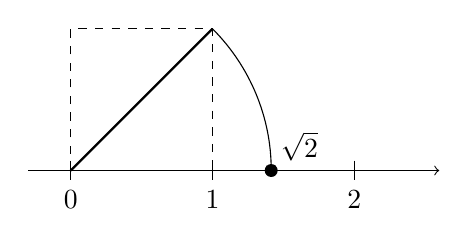
\begin{tikzpicture}[scale=1.8]
  \draw[->] (-0.3,0) -- (2.6,0);
  \foreach \x in {0,1,2} \draw (\x,0.07) -- (\x,-0.07) node[below] {$\x$};
  \draw[dashed] (0,0) rectangle (1,1);
  \draw[thick] (0,0) -- (1,1);
  \draw[->, thin] (1,1) arc (45:0:1.4142);
  \fill (1.4142,0) circle (1.3pt) node[above right] {$\sqrt{2}$};
\end{tikzpicture}

{\small La diagonal del cuadrado de lado 1 mide $\sqrt{2}$; el compás la lleva a la recta.}
\end{center}

\subsubsection*{La espiral de Teodoro}

Si sobre la hipotenusa $\sqrt{2}$ levantamos un cateto perpendicular de
longitud $1$, la nueva hipotenusa mide $\sqrt{(\sqrt{2})^2 + 1^2} =
\sqrt{3}$; repitiendo, aparecen $\sqrt{4} = 2$, $\sqrt{5}$, $\sqrt{6}$\ldots
Esta cadena de triángulos se llama hoy \emph{espiral de Teodoro}, en honor
del maestro de Platón; el nombre es moderno, y no sabemos si él la
usó~\cite{davis}.

\begin{center}
\begin{tikzpicture}[scale=1.3, every node/.style={font=\small}]
  \coordinate (O) at (0,0);
  \coordinate (P1) at (0:1);
  \coordinate (P2) at (45:1.4142);
  \coordinate (P3) at (80.264:1.7321);
  \coordinate (P4) at (110.264:2);
  \coordinate (P5) at (136.829:2.2361);
  \coordinate (P6) at (160.924:2.4495);
  \draw[thick] (P1) -- (P2) -- (P3) -- (P4) -- (P5) -- (P6);
  \foreach \p/\t in {P1/1, P2/\sqrt{2}, P3/\sqrt{3}, P4/2, P5/\sqrt{5}, P6/\sqrt{6}}
    \draw (O) -- (\p);
  \draw (O) -- (P1);
  \node[below] at ($(O)!0.5!(P1)$) {$1$};
  \node[right] at ($(P1)!0.5!(P2)$) {$1$};
  \node[above right] at ($(P2)!0.5!(P3)$) {$1$};
  \node[above] at ($(P3)!0.5!(P4)$) {$1$};
  \node[above left] at ($(P4)!0.5!(P5)$) {$1$};
  \node[left] at ($(P5)!0.5!(P6)$) {$1$};
  \node[fill=white, inner sep=1pt] at ($(O)!0.55!(P2)$) {$\sqrt{2}$};
  \node[fill=white, inner sep=1pt] at ($(O)!0.6!(P3)$) {$\sqrt{3}$};
  \node[fill=white, inner sep=1pt] at ($(O)!0.6!(P4)$) {$2$};
  \node[fill=white, inner sep=1pt] at ($(O)!0.6!(P5)$) {$\sqrt{5}$};
  \node[fill=white, inner sep=1pt] at ($(O)!0.6!(P6)$) {$\sqrt{6}$};
\end{tikzpicture}
\end{center}

Un mismo número tiene varias representaciones: $\sqrt{2}$ es la diagonal del
cuadrado de lado $1$, es el decimal $\num{1,41421356}\ldots$ (infinito y no
periódico) y es el número positivo cuyo cuadrado es $2$. Demostrar que
$\sqrt{2}$ no es fracción cabe en media página; con $\pi$ costó dos mil años
más.

\begin{aplicacion}[La hoja A4]
Las hojas A4, A3, A5\ldots\ de la norma internacional ISO 216 tienen una
razón entre largo y ancho de $\sqrt{2}$: es la única proporción que se
conserva al doblar la hoja por la mitad, y por eso una fotocopiadora reduce
una A3 a A4 sin deformar la imagen~\cite{iso216}. La hoja carta que se usa en
Colombia ($21{,}6 \times 27{,}9$ cm) no sigue esa norma.
\end{aplicacion}

\begin{preguntas}
% Ejercicio: irracionales-8-009 — manual-pendiente: entra cuando la docente
% apruebe la respuesta modelo (python3 tools/ejercicios.py aprobar irracionales-8-009).
% \pregunta Adapta la demostración de que $\sqrt{2}$ no es racional para
% probar que $\sqrt{3}$ tampoco lo es. (Pista: si $p^2 = 3q^2$, ¿qué puedes
% decir de $p$?)
% \espacio{3.5cm}
% Ejercicio: numeros-reales-8-001, numeros-reales-8-004, numeros-reales-8-006
\pregunta Representa en la recta real el número que resulta de cada operación:
\begin{opciones*}(3)
  \item $2 + \sqrt{2}$
  \item $\sqrt{5} - \sqrt{3}$
  \item $\dfrac{\sqrt{2}}{2} - 1$
\end{opciones*}
\espacio{3cm}
% Ejercicio: irracionales-8-011
\pregunta En la espiral de Teodoro, cada triángulo rectángulo tiene un
cateto de $1$ y el otro igual a la hipotenusa del triángulo anterior; el
primero tiene catetos $1$ y $1$. Calcula la hipotenusa de los cinco primeros
triángulos y di cuáles son números racionales.
\espacio{3cm}
% Ejercicio: irracionales-8-012
\pregunta Una hoja A4 mide $210 \times 297$ mm y una hoja carta,
$216 \times 279$ mm. Calcula la razón largo/ancho de cada una y compárala con
$\sqrt{2}$. Luego dobla cada hoja por la mitad (la mitad del largo) y calcula
de nuevo la razón. ¿Cuál conserva su forma?
\espacio{3.5cm}
% Ejercicio: irracionales-8-013
\pregunta Las fracciones $\dfrac{7}{5}$, $\dfrac{17}{12}$ y $\dfrac{99}{70}$
se acercan cada vez más a $\sqrt{2}$. Eleva cada una al cuadrado y compara
con $2$; luego calcula, con la calculadora, cuánto se aleja cada una de
$\sqrt{2}$.
\espacio{3.5cm}
\end{preguntas}

\begin{resumen}
\begin{itemize}
  \item $\sqrt{2}$ no es racional: se demuestra por el absurdo, suponiendo
        que sí lo es y llegando a una contradicción.
  \item Irracionales ($\I$): decimales infinitos no periódicos; no se pueden
        escribir como fracción.
  \item Algunos irracionales, como $\sqrt{2}$, $\sqrt{3}$ o $\sqrt{5}$, se
        construyen y se ubican exactamente en la recta con regla y compás.
\end{itemize}
\end{resumen}

% ---------------------------------------------------------------------
\tema{Los irracionales en la vida real}\label{tema:irracionalesvidareal}

\begin{hilo}
Ahora sí, la presa principal. $\pi$ aparece en cada rueda, cada tubo y cada
pista atlética. El papiro Rhind, Arquímedes y Zu Chongzhi lo aproximaron con
fracciones cada vez mejores; Lambert demostró que ninguna lo alcanza.
\end{hilo}

\begin{ejemplo}[Tres irracionales famosos]
\begin{itemize}
  \item $\pi \approx \num{3,14159}\ldots$: la razón entre la circunferencia
        de cualquier círculo y su diámetro.
  \item $e \approx \num{2,71828}\ldots$: aparece en el crecimiento continuo
        (poblaciones, interés compuesto).
  \item $\varphi = \dfrac{1 + \sqrt{5}}{2} \approx \num{1,61803}\ldots$ (la
        razón áurea): la razón entre la diagonal y el lado de un pentágono
        regular.
\end{itemize}
Ninguno de los tres es una fracción, aunque cada uno tiene una definición
exacta. Sus aproximaciones —$\frac{22}{7}$ para $\pi$, por ejemplo— sí son
fracciones: sirven para calcular, pero no son el número.
\end{ejemplo}

Juntando racionales e irracionales obtenemos los \textbf{números reales}:
$\R = \Q \cup \I$. Todo número real es racional o irracional, nunca las dos
cosas. Los conjuntos que ya conoces forman una cadena,
\[
  \N \subset \Z \subset \Q \subset \R,
\]
y $\I$ no está dentro de ella: es lo que le falta a $\Q$ para completar $\R$.

% Ejercicio: irracionales-8-019 (propiedad de la explicación; respuesta
% modelo pendiente de aprobación de la docente)
\begin{ejemplo}[Sumar y multiplicar racionales e irracionales]
Un racional más un irracional siempre da irracional: si $r + a = s$, con $r$
y $s$ racionales, entonces $a = s - r$ también sería racional. Pero dos
irracionales sí pueden dar un racional: $\sqrt{2} \cdot \sqrt{2} = 2$.
\end{ejemplo}

% Ejercicio: irracionales-8-017
\begin{aplicacion}[La rueda de una bicicleta]
Una rueda de $66$ cm de diámetro avanza en cada vuelta $66\pi \approx
\num{207,3}$ cm. Para recorrer $1$ km ($\num{100000}$ cm) da unas
$\num{100000} \div 66\pi \approx \num{482,3}$ vueltas. El cuentakilómetros
cuenta vueltas y las multiplica por la circunferencia; si usara
$\frac{22}{7}$ en lugar de $\pi$, contaría unos $\num{0,4}$ m de más por
cada kilómetro, un error del $\num{0,04}\,\%$.
\end{aplicacion}

\begin{preguntas}
% Ejercicio: irracionales-8-014
\pregunta Tres aproximaciones históricas de $\pi$ son $\dfrac{256}{81}$
(papiro Rhind, Egipto), $\dfrac{22}{7}$ (Arquímedes) y $\dfrac{355}{113}$
(Zu Chongzhi, China). Escribe cada una como decimal con siete cifras y di
cuántas cifras decimales coinciden con $\pi = \num{3,1415926}\ldots$
\espacio{3cm}
% Ejercicio: irracionales-8-015
\pregunta Clasifica cada número como natural, entero, racional o irracional
(puede pertenecer a varios conjuntos):
\begin{opciones*}(3)
  \item $\sqrt{9}$
  \item $\sqrt{7}$
  \item $-\dfrac{4}{2}$
  \item $\dfrac{22}{7}$
  \item $\pi$
  \item $2{,}101001000100001\ldots$ (cada vez un cero más entre los unos)
\end{opciones*}
\espacio{3cm}
% Ejercicio: irracionales-8-016
\pregunta ¿Es siempre irracional el resultado de sumar dos números
irracionales? Calcula $\sqrt{2} + \sqrt{2}$ y $\sqrt{2} + (3 - \sqrt{2})$ y
explica qué observas.
\espacio{3cm}
% Ejercicio: numeros-reales-8-025, numeros-reales-8-026
\pregunta Verifica con una calculadora que $\sqrt{5 + 4} \neq \sqrt{5} +
\sqrt{4}$ y que $\sqrt{5 - 4} \neq \sqrt{5} - \sqrt{4}$. ¿Qué concluyes sobre
la raíz de una suma?
\espacio{3cm}
% Ejercicio: irracionales-8-018
\pregunta Una llanta de carro tiene $58$ cm de diámetro. ¿Cuántas vueltas da
al recorrer $1$ km? Redondea a la vuelta más cercana y explica por qué aquí
tiene sentido redondear.
\espacio{2.5cm}
\end{preguntas}

\begin{resumen}
\begin{itemize}
  \item $\R = \Q \cup \I$: todo número real es racional o irracional, nunca
        ambos.
  \item $\pi$, $e$ y $\varphi$ son irracionales; $\frac{256}{81}$,
        $\frac{22}{7}$ y $\frac{355}{113}$ son aproximaciones racionales de
        $\pi$, cada vez mejores.
  \item Racional $+$ irracional es siempre irracional; dos irracionales
        pueden sumar o multiplicar a un racional.
\end{itemize}
\end{resumen}

% ---------------------------------------------------------------------
\tema{Radicales y aplicaciones}\label{tema:radicalesaplicaciones}

\begin{hilo}
Para encerrar a $\pi$ con sus polígonos, Arquímedes tuvo que calcular con
raíces cuadradas, como $\sqrt{3}$. Para usar los radicales en medidas reales
hay que saber simplificarlos y aproximarlos.
\end{hilo}

Para $a, b \ge 0$: $\sqrt{a \cdot b} = \sqrt{a} \cdot \sqrt{b}$. Esta
propiedad permite \textbf{simplificar} un radical sacando de la raíz los
factores que son cuadrados perfectos. Si el radicando es un entero sin
factores cuadrados perfectos (como $\sqrt{7}$ o $\sqrt{21}$), el radical ya
está simplificado y su valor es irracional.

% Ejercicio: irracionales-8-020
\begin{ejemplo}[Simplificar un radical]
\[
  \sqrt{50} = \sqrt{25 \cdot 2} = \sqrt{25} \cdot \sqrt{2} = 5\sqrt{2}.
\]
Los radicales con el mismo radicando se suman como términos semejantes:
$5\sqrt{2} + 3\sqrt{2} = 8\sqrt{2}$. En cambio, la raíz \emph{no} se reparte
en una suma: $\sqrt{9 + 16} = 5$, pero $\sqrt{9} + \sqrt{16} = 7$.
\end{ejemplo}

% Ejercicio: irracionales-8-023
\begin{ejemplo}[El primer encierro de $\pi$]
En un círculo de radio $1$ dibujamos un hexágono regular por dentro (lado
$1$) y otro por fuera (lado $\frac{2}{\sqrt{3}}$). La circunferencia, $2\pi$,
queda entre los dos perímetros:
\[
  6 < 2\pi < 6 \cdot \frac{2}{\sqrt{3}} = \frac{12}{\sqrt{3}} = 4\sqrt{3},
  \qquad\text{así que}\qquad 3 < \pi < 2\sqrt{3} \approx \num{3,46}.
\]
Arquímedes hizo lo mismo, pero duplicando los lados hasta llegar a 96.
\end{ejemplo}

\begin{center}
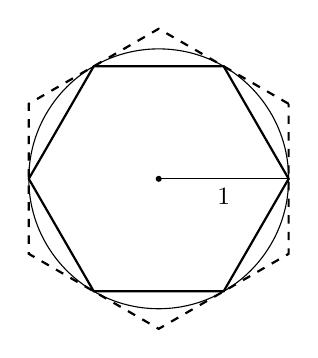
\begin{tikzpicture}[scale=1.1]
  \draw (0,0) circle (1.5);
  \draw[thick] (0:1.5) \foreach \a in {60,120,...,300} { -- (\a:1.5) } -- cycle;
  \draw[thick, dashed] (30:1.7321) \foreach \a in {90,150,...,330} { -- (\a:1.7321) } -- cycle;
  \fill (0,0) circle (1pt);
  \draw (0,0) -- node[below, font=\small] {$1$} (0:1.5);
\end{tikzpicture}

{\small Hexágono inscrito (línea continua) y circunscrito (línea discontinua).}
\end{center}

\begin{aplicacion}[El tamaño de un televisor]
Los televisores se anuncian por la medida de su \textbf{diagonal}, en
pulgadas. Una pantalla panorámica tiene razón ancho\,:\,alto de $16:9$; si el
ancho es $16k$ y el alto $9k$, la diagonal mide
$\sqrt{(16k)^2 + (9k)^2} = \sqrt{337}\,k \approx \num{18,36}\,k$. Para un
televisor de $32$ pulgadas, $k \approx \num{1,743}$: el ancho es de unas
$\num{27,9}$ pulgadas y el alto de unas $\num{15,7}$.
\end{aplicacion}

\begin{preguntas}
% Ejercicio: irracionales-8-020
\pregunta Simplifica:
\begin{opciones*}(3)
  \item $\sqrt{18}$
  \item $\sqrt{75}$
  \item $\sqrt{200}$
\end{opciones*}
\espacio{3cm}
% Ejercicio: irracionales-8-021
\pregunta Camila dice: «$\sqrt{18} + \sqrt{2} = \sqrt{20}$, porque sumé lo
de adentro de la raíz». ¿Estás de acuerdo? Simplifica cada radical por
separado y muestra el procedimiento correcto.
\espacio{3cm}
% Ejercicio: radicacion-8-034
\pregunta Simplifica la expresión $5\sqrt{2} + 8\sqrt{3} + 9\sqrt{2} - \sqrt{3}$.
\espacio{2cm}
% Ejercicio: irracionales-8-022
\pregunta Para encerrar a $\pi$, Arquímedes usó que $\dfrac{265}{153} <
\sqrt{3} < \dfrac{1351}{780}$. Compruébalo sin calculadora elevando al
cuadrado (compara $265^2$ con $3 \cdot 153^2$, y $1351^2$ con
$3 \cdot 780^2$). Luego, con la calculadora, di cuántas cifras decimales de
$\sqrt{3} = \num{1,7320508}\ldots$ acierta cada fracción.
\espacio{3.5cm}
% Ejercicio: irracionales-8-024
\pregunta Una escalera de $5$ m se apoya contra una pared, con la base a
$2$ m del muro. ¿A qué altura llega? Da el resultado exacto (radical
simplificado) y una aproximación con dos cifras decimales.
\espacio{3cm}
% Ejercicio: irracionales-8-025
\pregunta Calcula la diagonal exacta de un jardín rectangular de $6$ m por
$4$ m y la de uno de $3$ m por $4$ m. ¿Por qué una es racional y la otra no?
\espacio{3cm}
% Ejercicio: medidas-con-radicales-8-001
\pregunta Encuentra el perímetro de un triángulo rectángulo isósceles cuyos
catetos miden $5$~cm.
\espacio{2.5cm}
\end{preguntas}

\begin{resumen}
\begin{itemize}
  \item $\sqrt{a \cdot b} = \sqrt{a} \cdot \sqrt{b}$ para $a, b \ge 0$: así se
        simplifica un radical sacando los cuadrados perfectos.
  \item Solo se suman radicales con el mismo radicando; la raíz de una suma
        no es la suma de las raíces.
  \item Una raíz se puede encerrar entre dos fracciones comparando sus
        cuadrados, como hizo Arquímedes con $\sqrt{3}$ para encerrar a $\pi$.
\end{itemize}
\end{resumen}

% ---------------------------------------------------------------------
% 5. Cierre del hilo conductor
% ---------------------------------------------------------------------
\seccion{Cierre: cuatro mil años de cacería}

Del $3{,}16$ del papiro Rhind al $\frac{22}{7}$ de Arquímedes, al
$\frac{355}{113}$ de Zu Chongzhi, a la demostración de Lambert de que
ninguna fracción es $\pi$, y a los 314 billones de cifras de hoy. La lección
matemática de esta historia es que hay números que no caben en ninguna
fracción y que, aun así, podemos construirlos, ubicarlos en la recta y
calcularlos con la precisión que haga falta. Y hay otra lección: de muchos
personajes antiguos sabemos poco y se cuenta mucho, pero una demostración,
como la de $\sqrt{2}$, cualquiera la puede repetir y comprobar. En el
siguiente trimestre dejaremos los números fijos y trabajaremos con letras:
el lenguaje algebraico, las expresiones y las ecuaciones.

% ---------------------------------------------------------------------
% 6. Evaluación (secciones institucionales)
% ---------------------------------------------------------------------
\matrizevaluacion
  {Distingue racionales de irracionales por su expresión decimal; reconoce
   $\sqrt{2}$, $\pi$, $e$ y $\varphi$ y sabe por qué $\frac{22}{7}$ no es $\pi$.}
  {Demuestra que $\sqrt{2}$ no es racional; construye y ubica irracionales
   en la recta; simplifica y aproxima radicales en problemas de medidas.}
  {Revisa sus procedimientos y los de sus compañeros con argumentos, sin
   conformarse con «se ve que sí».}
  {Valora que la matemática avanza cuestionando lo que parecía evidente, y
   distingue lo demostrado de lo que solo se sospecha o se cuenta.}

\autoevaluacion

\seguimientodocente

% ---------------------------------------------------------------------
% 7. Referencias
% ---------------------------------------------------------------------
\begin{referencias}
% verificado: https://bibcatalogo.uca.es/cgi-bin/koha/opac-detail.pl?biblionumber=603122 — Gredos 1994, trad. T. Calvo Martínez, Biblioteca Clásica Gredos 200, ISBN 84-249-1666-2; pasaje pitagórico en Met. I.5
\bibitem{aristoteles} Aristóteles (1994). \emph{Metafísica} (trad. T. Calvo
  Martínez; Biblioteca Clásica Gredos, 200), libro I, cap. 5. Madrid: Gredos.
% verificado: https://arxiv.org/pdf/1101.0492 — Arquímedes usa 265/153 < √3 < 1351/780 en La medida del círculo (polígonos de 96 lados) sin explicar cómo lo obtuvo
\bibitem{arqraices} Archimedes' calculations of square roots (2011).
  \emph{arXiv}:1101.0492. \url{https://arxiv.org/abs/1101.0492}
% verificado: https://www.tau.ac.il/~corry/publications/articles/Narrative/notes/aristo.html — Primeros analíticos I.23: la diagonal inconmensurable, «odd numbers are equal to evens»
\bibitem{corry} Corry, L. \emph{Aristotle on incommensurability} (nota).
  Universidad de Tel Aviv. \url{https://www.tau.ac.il/~corry/}
% verificado: https://books.google.com.co/books/about/Spirals.html?id=eEbvAAAAMAAJ — Davis, Gautschi, Iserles, 1993, 237 pp.; Davis nombra la ecuación en diferencias por Teodoro
\bibitem{davis} Davis, P. J. (1993). \emph{Spirals: From Theodorus to Chaos}
  (con W. Gautschi y A. Iserles). Taylor \& Francis.
% verificado: https://bmcr.brynmawr.edu/1995/1995.07.07/ — reseña BMCR de Dzielska, Hypatia of Alexandria, Harvard UP 1995 (Revealing Antiquity 8, trad. F. Lyra); comentarios a Diofanto y Apolonio en https://mathshistory.st-andrews.ac.uk/Biographies/Hypatia/
\bibitem{dzielska} Dzielska, M. (1995). \emph{Hypatia of Alexandria} (trad.
  F. Lyra). Cambridge, MA: Harvard University Press.
% verificado: https://mathcs.clarku.edu/~djoyce/elements/bookX/bookX.html — Libro X, 115 proposiciones sobre magnitudes conmensurables e inconmensurables
\bibitem{euclides} Euclides (ca. 300 a.\,C.). \emph{Elementos}, Libro X
  (edición electrónica de D. E. Joyce, Clark University, a partir de la
  traducción de T. L. Heath).
% verificado: https://plato.stanford.edu/archives/fall2020/entries/pythagoreanism/ — ninguna fuente antigua liga a Hipaso con el descubrimiento de los irracionales; Jámblico lo castiga por divulgar el dodecaedro
\bibitem{huffman} Huffman, C. (2020). Pythagoreanism. En E. N. Zalta (ed.),
  \emph{Stanford Encyclopedia of Philosophy} (ed. otoño 2020).
% verificado: https://www.cl.cam.ac.uk/~mgk25/iso-paper.html — ISO 216: razón √2, se conserva al cortar por la mitad; A0 = 1 m²
\bibitem{iso216} Kuhn, M. \emph{International standard paper sizes (ISO 216)}.
  Universidad de Cambridge. \url{https://www.cl.cam.ac.uk/~mgk25/iso-paper.html}
% verificado: https://link.springer.com/book/10.1007/978-1-4757-4217-6 — Pi: A Source Book, 3.ª ed., Springer 2004, memoria de Lambert pp. 129-140; presentada en 1761 según https://mathshistory.st-andrews.ac.uk/HistTopics/Pi_through_the_ages/
\bibitem{lambert} Lambert, J. H. (1768/2004). Mémoire sur quelques propriétés
  remarquables des quantités transcendantes circulaires et logarithmiques.
  En L. Berggren, J. Borwein y P. Borwein (eds.), \emph{Pi: A Source Book}
  (3.\textsuperscript{a} ed., pp. 129--140). Nueva York: Springer.
% verificado: https://mathshistory.st-andrews.ac.uk/HistTopics/Pi_through_the_ages/ — Rhind (~1650 a. C., 4·(8/9)² ≈ 3,16); Arquímedes 223/71 < π < 22/7; Zu Chongzhi (430-501) 355/113; Lambert 1761
\bibitem{mactutorpi} O'Connor, J. J. y Robertson, E. F. \emph{A history of Pi}.
  MacTutor History of Mathematics, Universidad de St Andrews.
% verificado: https://mathshistory.st-andrews.ac.uk/Biographies/Theodorus/ — cita Teeteto 147d: raíces de 3, 5… hasta 17 inconmensurables con la unidad
\bibitem{mactutortheodorus} O'Connor, J. J. y Robertson, E. F. \emph{Theodorus
  of Cyrene}. MacTutor History of Mathematics, Universidad de St Andrews.
% verificado: https://gblumen.mineducacion.gov.co/cgi-bin/koha/opac-detail.pl?biblionumber=4785 — MEN 2016, ISBN 978-958-691-913-5
\bibitem{mendba} Ministerio de Educación Nacional (2016). \emph{Derechos
  Básicos de Aprendizaje V.2: Matemáticas}. Bogotá: MEN.
% verificado: https://www.guinnessworldrecords.com/news/commercial/2026/6/pi-high-computing-achievement-technology-companies-calculate-pi-to-340-trillionth-digit — récord vigente (junio 2026): 314 billones de cifras, StorageReview y Micron, 110 días; anuncio en https://www.storagereview.com/review/storagereview-sets-new-pi-record-314-trillion-digits-on-a-dell-poweredge-r7725
\bibitem{storagereview} StorageReview (2025). \emph{StorageReview Sets New Pi
  Record: 314 Trillion Digits on a Dell PowerEdge R7725}.
  \url{https://www.storagereview.com}
\end{referencias}

\end{document}
